\chapter{\IfLanguageName{dutch}{Stand van zaken}{State of the art}}%
\label{ch:stand-van-zaken}

% Tip: Begin elk hoofdstuk met een paragraaf inleiding die beschrijft hoe
% dit hoofdstuk past binnen het geheel van de bachelorproef. Geef in het
% bijzonder aan wat de link is met het vorige en volgende hoofdstuk.

% Pas na deze inleidende paragraaf komt de eerste sectiehoofding.

% Dit hoofdstuk bevat je literatuurstudie. De inhoud gaat verder op de inleiding, maar zal het onderwerp van de bachelorproef *diepgaand* uitspitten. De bedoeling is dat de lezer na lezing van dit hoofdstuk helemaal op de hoogte is van de huidige stand van zaken (state-of-the-art) in het onderzoeksdomein. Iemand die niet vertrouwd is met het onderwerp, weet nu voldoende om de rest van het verhaal te kunnen volgen, zonder dat die er nog andere informatie moet over opzoeken \autocite{Pollefliet2011}.

% Je verwijst bij elke bewering die je doet, vakterm die je introduceert, enz.\ naar je bronnen. In \LaTeX{} kan dat met het commando \texttt{$\backslash${textcite\{\}}} of \texttt{$\backslash${autocite\{\}}}. Als argument van het commando geef je de ``sleutel'' van een ``record'' in een bibliografische databank in het Bib\LaTeX{}-formaat (een tekstbestand). Als je expliciet naar de auteur verwijst in de zin (narratieve referentie), gebruik je \texttt{$\backslash${}textcite\{\}}. Soms is de auteursnaam niet expliciet een onderdeel van de zin, dan gebruik je \texttt{$\backslash${}autocite\{\}} (referentie tussen haakjes). Dit gebruik je bv.~bij een citaat, of om in het bijschrift van een overgenomen afbeelding, broncode, tabel, enz. te verwijzen naar de bron. In de volgende paragraaf een voorbeeld van elk.

% \textcite{Knuth1998} schreef een van de standaardwerken over sorteer- en zoekalgoritmen. Experten zijn het erover eens dat cloud computing een interessante opportuniteit vormen, zowel voor gebruikers als voor dienstverleners op vlak van informatietechnologie~\autocite{Creeger2009}.

% Let er ook op: het \texttt{cite}-commando voor de punt, dus binnen de zin. Je verwijst meteen naar een bron in de eerste zin die erop gebaseerd is, dus niet pas op het einde van een paragraaf.

Om gebruik te maken van \textit{graphics processing unit} (\textit{GPU}) acceleratie is het vereist dat applicaties communiceren met een \textit{interface}. Zo bestaan er onderliggend in besturingssystemen \textit{GPU Application Programming Interfaces} (\textit{GPU API's}) zoals \textit{Direct3D} voor \textit{Microsoft Windows}, \textit{Metal} voor ontwikkeling op het \textit{Apple} ecosysteem en \textit{Vulcan} als open standaard \autocite{Nguyen2022}. Dit zijn complexe software oplossingen die de beste prestaties bieden en hierdoor toelaten dat software optimaal gebruik kan maken van de onderliggende \textit{hardware}. Het is echter duidelijk dat het onderhouden van software voor verschillende besturingssystemen complex is en veel energie vergt, wat ervoor zorgt dat applicaties vaak maar beperkt worden ondersteund. Dit is een probleem dat \textit{WebGPU} verhelpt door een abstractielaag te vormen boven deze \textit{APIs}~\autocite{Wallez2023}.

\section{Rekenkracht op het web}
\label{sec:PowerOnWeb}

Rekenkundige taken op het web werden voorheen in beperkte mate uitgevoerd met \textit{WebGL}. Deze technologie is gebaseerd op de OpenGL standaard. \textit{WebGL 2.0} laat toe om berekeningen uit te voeren en hierbij de parallelle rekenkracht van grafische processoren te gebruiken. Wanneer de grafische rekenkracht van een \textit{GPU} wordt ingezet om algemene calculaties uit te voeren wordt de term \textit{general purpose graphics processing unit} gebruikt ook wel \textit{GPGPU}~\autocite{Skrbina2012}.

\begin{displayquote}[{\cite{Tavares2021}}]
    "The basic realization to understanding GPGPU in WebGL is that a texture is not an image, it's a 2D array of values."
\end{displayquote}

\begin{figure}
    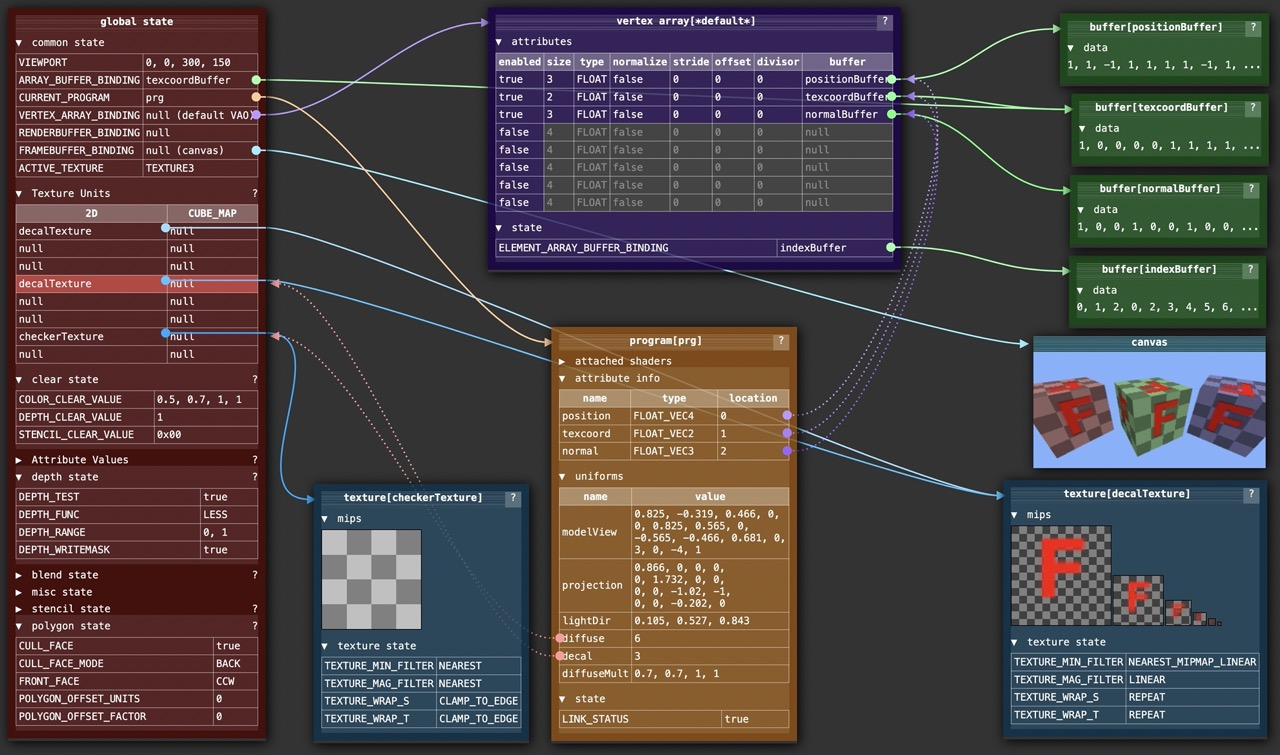
\includegraphics[width=\linewidth]{WebGLAndGlobalState.jpeg}
    \caption[De \textit{Global State} in \textit{WebGL}~\autocite{GFXFundamentals2024}]{Gebruik van een globale variable binnen WebGL~\autocite{GFXFundamentals2024}.}
    \label{fig:WebGL Global State}
\end{figure}

\textit{WebGL} gebruiken voor \textit{GPGPU} is echter een complexe implementatie die gebruik maakt van een \textit{global state} die volgens \textcite{Surma2022} al snel kan leiden tot een complexe code, en hierdoor ook tot fouten. Een schematische voorstelling van deze \textit{global state} wordt weergegeven in figuur \ref{fig:WebGL Global State}. De implementatie van \textit{GPGPU} werd door de introductie van \textit{Transform Feedback} in \textit{WebGL 2.0} toegankelijker. Dit is een simpelere methode om de data uit te lezen na een complexe berekening op de grafische kaart aan de hand van \textit{WebGL}. De data zit namelijk in een eendimensionale waardoor hier makkelijker verder mee te werken is~\autocite{Tavares2021}. Maar deze nieuwere versie van \textit{WebGL} werd pas in september 2021 ondersteund door \textit{Apple} op \textit{Safari}~\autocite{Surma2022}.

\bigbreak{}

\textit{WebGPU} vervangt dit \textit{global state} gedrag met \textit{pipelines} die niet aanpasbaar zijn. En omdat \textit{compute shaders} beschikbaar zijn is de \textit{Transform Feedback} oplossing niet meer nodig~\autocite{Beaufort2023}. Het gebruiken van WebGL voor \textit{GPGPU} is niet enkel complex, het is ook inefficiënt. Data moet eerst als een \textit{texture} worden gecodeerd, daarna worden gedecodeerd in een \textit{shader}. Op dat moment moeten de eigenlijke berekeningen worden uitgevoerd. De resultaten van deze berekeningen moeten daarna opnieuw worden gecodeerd tot een \textit{texture}, alvorens er met de data kan worden verder gewerkt~\autocite{Surma2022}.

\bigbreak{}

Deze lange onnodige complexiteit komt voort uit het feit dat \textit{WebGL} werd ontworpen voor het visualiseren van grafische elementen en niet om algemene computationele taken uit te voeren zoals \textit{machine learning} of het mijnen van \textit{crypto currency}. Zoals eerder vermeld verbeterde de situatie wel met \textit{WebGL 2.0}, maar de ondersteuning hiervoor was beperkt en hierdoor kwam de proliferatie van lokale rekenkracht in de browser niet tot stand.

\break{}

\section{Introductie van WebGPU}
\label{sec:IntroWebGPU}

Omdat \textit{WebGPU} wordt gestandaardiseerd door het \textit{World Wide Web Consortium}, krijgt het ook de nodige ondersteuning om een potentiële standaard te worden zoals \textit{WebGL}. Een globaal initiatief kan er toe leiden dat deze technologie een revolutie betekent voor grafische weergave en voor lokale rekenkracht op het Web. In tegenstelling tot de beperkte ondersteuning waar \textit{WebGL 2.0} op kon rekenen, zitten bij \textit{WebGPU} wel alle browserfabrikanten mee in het ontwikkelingsproces~\autocite{Surma2022}.

\bigbreak{}

De werking van een GPU is heel complex. Hier wordt vaak te snel over gegaan. Er wordt door meerdere applicaties simultaan data naar het beeldscherm geprojecteerd waarbij de grafische kaart wordt opgedeeld. De veiligheidsimplicaties hiervan zijn niet te onderschatten, omdat deze applicaties elkaar niet mogen kunnen beïnvloeden of data van elkaar mogen uitlezen. Voor elke applicatie lijkt het dat deze over een monopolie beschikt van een grafische kaart. Uiteraard is dit niet het geval en wordt eigenlijk de rekenkracht verdeeld. Dit leidt ertoe dat de status van uitgevoerde taken moet worden bijgehouden omdat er altijd parallel wordt gewerkt. Programmeren voor \textit{General Purpose GPU} verloopt altijd op een \textit{multithreaded} asynchrone manier, waar rekening mee moet gehouden worden~\autocite{Surma2022}.

\bigbreak{}

Uiteraard zijn er al meerdere implementaties van \textit{machine learning} op het web, maar deze worden beschikbaar gesteld door servers en er wordt nog geen gebruik gemaakt van \textit{client-sided WebGPU rendering}. \textcite{Fleetwood2023a} beweert dat het essentieel zal zijn dat modellen lokaal worden gedraaid om de echte \textit{real time} te ondersteunen. Ook wanneer meerdere AI-modellen serieel worden gebruikt, om de functionaliteit van webapplicaties uit te breiden, verhoogt de vraag naar rekencapaciteit.

\bigbreak{}

Ook \textcite{Huyen2023} merkt in haar onderzoek op dat de kost van het draaien van AI-modellen in een productieomgeving enorm hoog kan oplopen. Hierdoor komt de rendabiliteit in gevaar. Dit is echter enkel het geval wanneer modellen suboptimaal worden ingezet zoals \textcite{Fleetwood2023a} opmerkt.

\begin{displayquote}[{\cite{Fleetwood2023a}}]
    "Offloading some parts of the call chain to finetuned local models could dramatically reduce costs while offering additional benefits such as privacy and personalization."
\end{displayquote}

\bigbreak{}

De programmeertaal die wordt gebruikt om code uit te voeren op de GPU aan de hand van WebGPU heet de \textit{WebGPU Shading Language} (\textit{WGSL}) \autocite{W3C2024}. Deze taal werd al reeds opgemerkt als een moeilijke programmeertaal om mee te werken~\autocite{Madrigal2023, Ashton2020}. Volgens \textcite{Fleetwood2023a} is dit echter niet het geval. Hij vindt namelijk dat de syntax toegankelijk is omdat het veel invloeden heeft van \textit{Rust}, een populaire opkomende taal. Wanneer \textit{shaders} worden geprogrammeerd voor \textit{WebGPU} moet dit gebeuren aan de hand van \textit{WGSL} implementaties.

\bigbreak{}

\textit{WebGPU} laat toe dat er rekenkracht beschikbaar wordt gesteld aan de browser maar dit wil niet zeggen dat hiermee het probleem van de werking van complexe modellen lokaal in de browser is opgelost. Er is namelijk ook een geheugenlimiet omdat een model moet worden ingeladen. Hiervoor gaat de voorkeur naar het gebruik van het geheugen van de grafische kaart, indien deze te klein is geeft dit merkbare prestatiebeperkingen. Er kan hierdoor potentieel een \textit{bottleneck} ontstaan. Het efficiënt inladen en beschikbaar stellen van deze modellen is essentieel.

\section{WebGPU in vergelijking met WebGL}

Uit de ondervindingen van \textcite{Radin2021} blijkt dat \textit{WebGPU} tot drie maal sneller kan zijn dan \textit{WebGL} in simpele matrix multiplicatie. Dit komt enerzijds omdat het proces om de berekeningen uit te voeren met \textit{WebGPU} een stuk eenvoudiger is, maar ook omdat \textit{WebGPU} \textit{compute shaders} ondersteunt in tegenstelling tot \textit{WebGL}. Om berekeningen uit te voeren met \textit{WebGL} is het namelijk vereist dat de data eerst worden omgezet naar pixels zodat deze met een \textit{pixel shader} kunnen worden berekend zoals eerder vermeld in sectie \ref{sec:PowerOnWeb}. 

\bigbreak{}

Nog een nadeel van de afhankelijkheid op de \textit{pixel shader} van \textit{WebGL} is dat er gebruik moet gemaakt worden van het canvas object. \textcite{Radin2021} ondervond dat \textit{WebGL} matrix multiplicatie niet ondersteunt boven de 4096 x 4096, \textit{WebGPU} kon echter berekeningen uitvoeren tot matrices van 5000 x 5000. Het is ook belangrijk hierbij op te merken dat berekeningen uitgevoerd met \textit{WebGPU} asynchroon zijn, wat eigen is aan grafische kaarten en \textit{GPGPU}, zoals eerder vermeld in sectie \ref{sec:IntroWebGPU}. Dit feit valt ook uit te lezen op basis van de resultaten van \textcite{Radin2021} in figuur \ref{fig:Matrix Multiplication By Radin} waarbij duidelijk is dat bij de \textit{JavaScript} implementatie berekeningen relatief tot de \textit{GPU} implementaties initieel sneller beginnen. De begrenzingen van rekenkracht met \textit{JavaScript} op de processor worden echter wel snel duidelijk: matrices kunnen niet meer worden uitgevoerd wanneer deze te groot zijn. Dit geldt ook voor de \textit{WebGL} implementatie maar dat is pas bij grotere matrices.

\bigbreak{}

De \textit{GPU} implementaties van de test van \textcite{Radin2021} blijven met grotere matrices verder werken. De verschillen tussen \textit{WebGPU} en \textit{WebGL} manifesteren zich wel in het uiteenlopen van de uitvoeringstijd. Hierbij stijgt de benodigde tijd voor \textit{WebGL} sneller dan die van \textit{WebGPU} voor identieke matrices. Dit komt onder andere omdat er geen conversie moet worden uitgevoerd van en naar de \textit{GPU buffer} bij \textit{WebGPU}, wat wel het geval is bij \textit{WebGL} zoals eerder vermeld in sectie \ref{sec:PowerOnWeb}. 

\break{}

\begin{figure}
    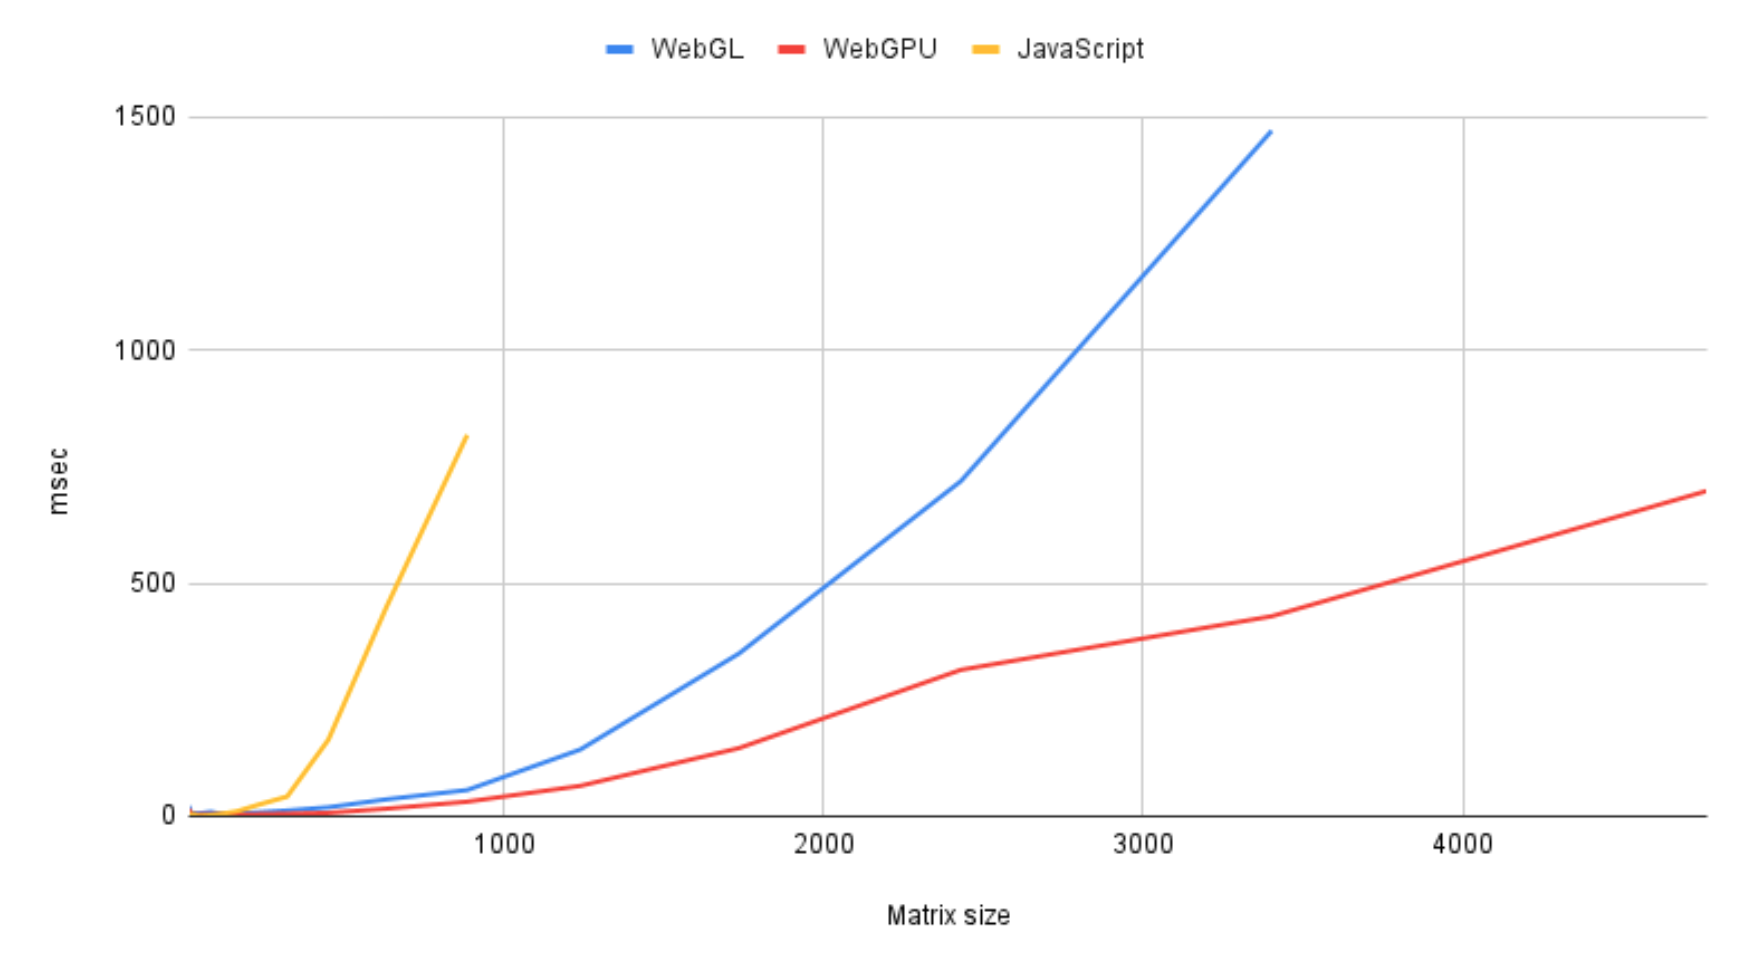
\includegraphics[width=\linewidth]{RadinMatrixMultiplicatie.png}
    \caption[Matrixvermenigvuldiging test~\autocite{Radin2021}]{Een test waarbij de prestaties van WebGPU, WebGL en \textit{JavaScript} worden vergeleken~\autocite{Radin2021}.}
    \label{fig:Matrix Multiplication By Radin}
\end{figure}

Het asynchrone gedrag en de efficiëntere implementatie van \textit{WebGPU} dragen bij aan het feit dat \textit{JavaScript} implementaties, die gebruik maken van \textit{WebGPU}, een lagere \textit{overhead} hebben. Dit betekent dat de achterliggende processor waarop \textit{JavaScript} code wordt uitgevoerd minder  belast wordt, omdat de zwaardere berekeningen worden uitbesteed aan de grafische kaart. Deze wordt beschikbaar gesteld door \textit{API's} zoals \textit{WebGL} en nu ook \textit{WebGPU}.

\begin{displayquote}[{\cite{Wallez2023}}]
    "As an example of the efficiency gains this can bring, an initial port of an image diffusion model in TensorFlow.js shows a 3x performance gain on a variety of hardware when moved from WebGL to WebGPU."
\end{displayquote}

De prestatieverbeteringen, die \textcite{Wallez2023} bij het gebruik van \textit{TensorFlow.js} opmerkt, worden niet enkel bevestigd wanneer er vergeleken wordt tussen \textit{WebGPU} en \textit{WebGL}. Ook in sectie \ref{sec:transformerbench} worden gelijkaardige resultaten behaald. De \textit{embedding} prestaties van zowel \textit{WebGPU} als \textit{Web Assembly} (\textit{WASM}), een compacte \textit{assembly-like binary} die prestaties op het web toelaat vergelijkbaar met \textit{native} talen zoals \textit{C/C++} en \textit{Rust} \autocite{Steiner2023}, werden hier met elkaar vergeleken.

\bigbreak{}

De ondervindingen van \textcite{Wallez2023} en \textcite{Radin2021} worden opnieuw bevestigd. De \textit{embedding} prestaties, een process waarbij data in een vector databank wordt verwerkt zodat hierbij verbindingen kunnen worden gelegd \autocite{Cloudflare2024, Cloudflare2024a, Huyen2023}, liggen hoger wanneer \textit{WebGPU} wordt vergeleken met een processor implementatie zoals \textit{WASM} voor \textit{use cases} zoals het trainen van AI-modellen.

\break{}

\section{Het nut van lokale rekenkracht in de browser} 

\textcite{Fleetwood2022} merkt op dat er een paradigma verandering aankomt in hoe AI-modellen worden getraind. De huidige technologie werkt als volgt: informatie wordt door de gebruiker voorzien en opgestuurd naar een model dat beschikbaar is in de \textit{cloud} en dit model produceert een antwoord dat terug aan de gebruiker wordt voorgelegd.

\bigbreak{}

Dit paradigma is enigszins statisch, omdat het model dat draait in de \textit{cloud} niet veranderlijk is. \textcite{Fleetwood2022} gelooft dat een standaard met modellen die dynamisch opgebouwd worden, de toekomst is. Dit wil zeggen dat gewichten die worden toegepast op een AI-model gepersonaliseerd zijn voor de gebruiker. 

\bigbreak{}

Wanneer gewichten worden toegepast op AI-modellen kan het gedrag worden aangepast. Omdat AI-modellen worden opgebouwd met een enorme hoeveelheid data die niet altijd perfect is, kunnen er kleine aanpassingen worden gedaan door parameters te veranderen. Hierbij worden gewichten toegevoegd aan zaken die relevanter zijn. Dit gebeurt bij het training process wanneer een AI-model wordt geoptimaliseerd~\autocite{Hubbard2024}.

\begin{displayquote}[{\cite{Fleetwood2022}}]
    "It would be optimal if the subset of weights that get updated to learn about the user remained on their device."
\end{displayquote}

Het is duidelijk dat gepersonaliseerde AI-modellen die dynamisch worden opgebouwd een impact hebben op de privacy- en veiligheidsaspecten. Deze aanpassingen kunnen gevoelige informatie bevatten en hiervan kan misbruik. Het gebruik maken van AI-modellen die niet lokaal werken kunnen mogelijks lekken veroorzaken van geheime of gevoelige bedrijfsinformatie~\autocite{Wiggers2023, Sabin2023}. Het valt op te merken dat lokale beschikbaarheid van rekenkracht op het web door middel van \textit{WebGPU} een katalysator kan zijn voor een  revolutionaire verandering in privacy en veiligheid op het web.

\bigbreak{}

Wat \textcite{Fleetwood2022} ook opmerkt is dat er bij het draaien van  AI-technologieën vaak meerdere processen serieel werken. Juist omdat er verder wordt gewerkt op informatie die reeds werd gegenereerd, leent deze technologie zich voor een tussenoplossing. Deze zou toestaan een hybride \textit{cloud} te maken waarbij een deel van de computationele taken worden overgedragen aan de eindgebruiker.

\bigbreak{}

Er moet nog wel worden benadrukt dat het downloaden van AI-modellen een groot struikelblok voor de technologie kan vormen. Veel AI-modellen worden niet publiek gemaakt waardoor geen gebruik kan worden gemaakt van een \textit{WebGPU} implementatie. AI-modellen die te groot zijn zorgen ervoor dat de eindgebruiker initieel moet wachten. Dit kan leiden tot een verminderde bruikbaarheid. Maar volgens \textcite{Fleetwood2022} zijn dit problemen die door middel van compressie en \textit{caching} grotendeels verholpen kunnen worden.

\break{}

\begin{figure}
    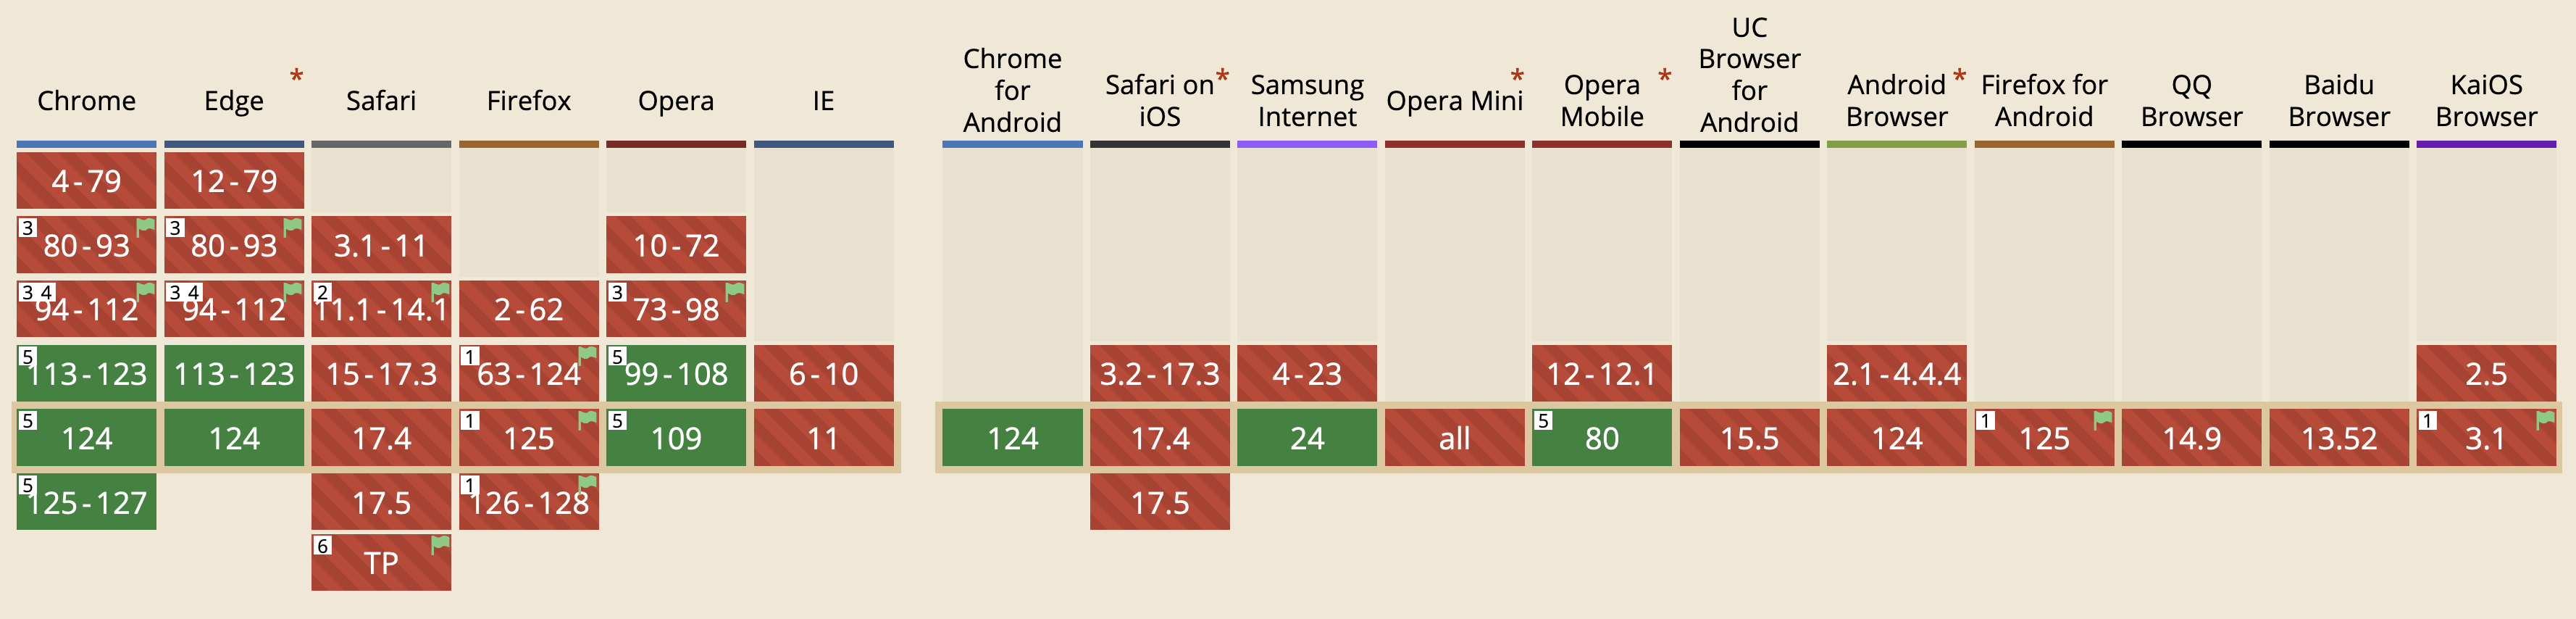
\includegraphics[width=\linewidth]{browsersupport.png}
    \caption[Ondersteuning voor \textit{WebGPU}~\autocite{Deveria2024}]{
        De \textit{Browser} ondersteuning voor \textit{WebGPU} te vinden op \href{https://caniuse.com/webgpu}{caniuse.com/webgpu}~\autocite{Deveria2024}.
    }
    \label{fig:Browser Support}
\end{figure}

\begin{figure}
    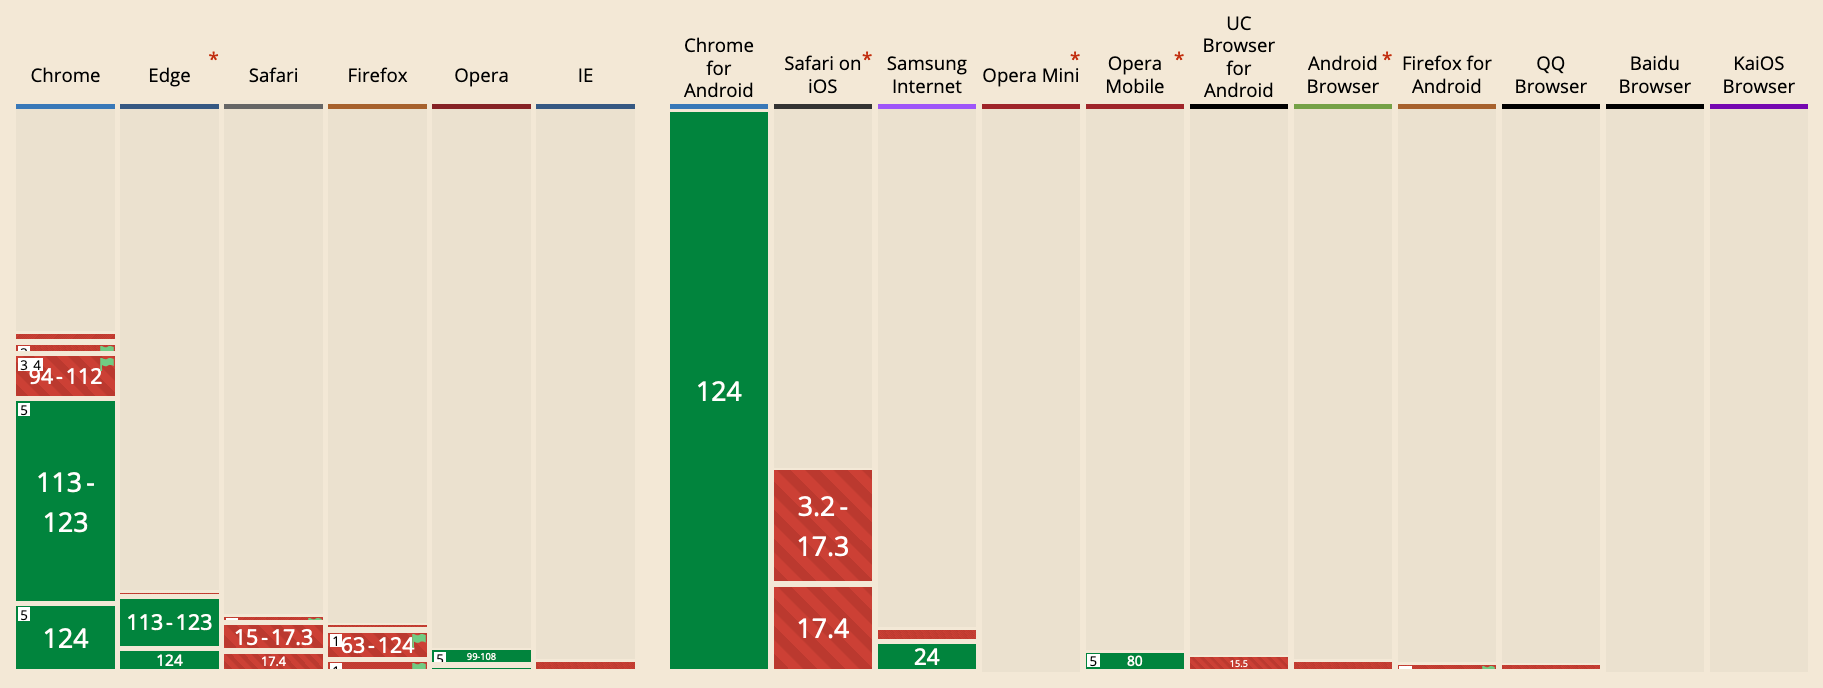
\includegraphics[width=\linewidth]{browsersupportuserrelative.png}
    \caption[Eindgebruikers met toegang tot \textit{WebGPU}~\autocite{Deveria2024}]{
        Ondersteuning voor \textit{WebGPU} te vinden op \href{https://caniuse.com/webgpu}{caniuse.com/webgpu} relatief tot gebruikers~\autocite{Deveria2024}.
    }
    \label{fig:Relative Browser Support}
\end{figure}

\section{WebGPU browser ondersteuning}

WebGPU wordt nog niet door alle \textit{browsers} ondersteund. Het is belangrijk dat de \textit{early adopter} gebruikers verifiëren of hun browser compatibel is. Dit kan makkelijk worden uitgezocht aan de hand van \href{https://caniuse.com/webgpu}{caniuse.com}. Omdat \textit{WebGPU} een relatief nieuwe technologie is, wordt deze soms enkel in testversies ondersteund. Zie \textit{Firefox} met groene vlagjes op afbeelding \ref{fig:Browser Support}. Merkwaardig is ook dat \textit{Chrome} volledige ondersteuning biedt op de desktop- en mobiele markt ~\autocite{Deveria2024}.

\bigbreak{}
\newdate{date}{06}{05}{2024}
\date{\displaydate{date}}

Afbeelding \ref{fig:Browser Support} toont de ondersteuning voor \textit{WebGPU} binnen verschillende \textit{browsers}: deze worden horizontaal weergegeven. De verschillende versies van specifieke \textit{browsers} worden verticaal opgelijst. Omdat er veel versies rood worden aangeduid zou kunnen worden afgeleid dat ondersteuning voor \textit{WebGPU} nog niet is doorgebroken, wat echter niet het geval is. Afbeelding \ref{fig:Relative Browser Support} toont een correcter beeld. De grafiek geeft een relatief beeld weer van de verdeling van het aantal gebruikers per \textit{browser} en versie. Op  \displaydate{date} heeft 70,51\% van de totale browser gebruikers toegang tot \textit{WebGPU}, volgens statistische informatie beschikbaar gesteld door \textcite{Deveria2024}.

\section{Realistisch scenario's simuleren met WebGPU}

\begin{figure}
    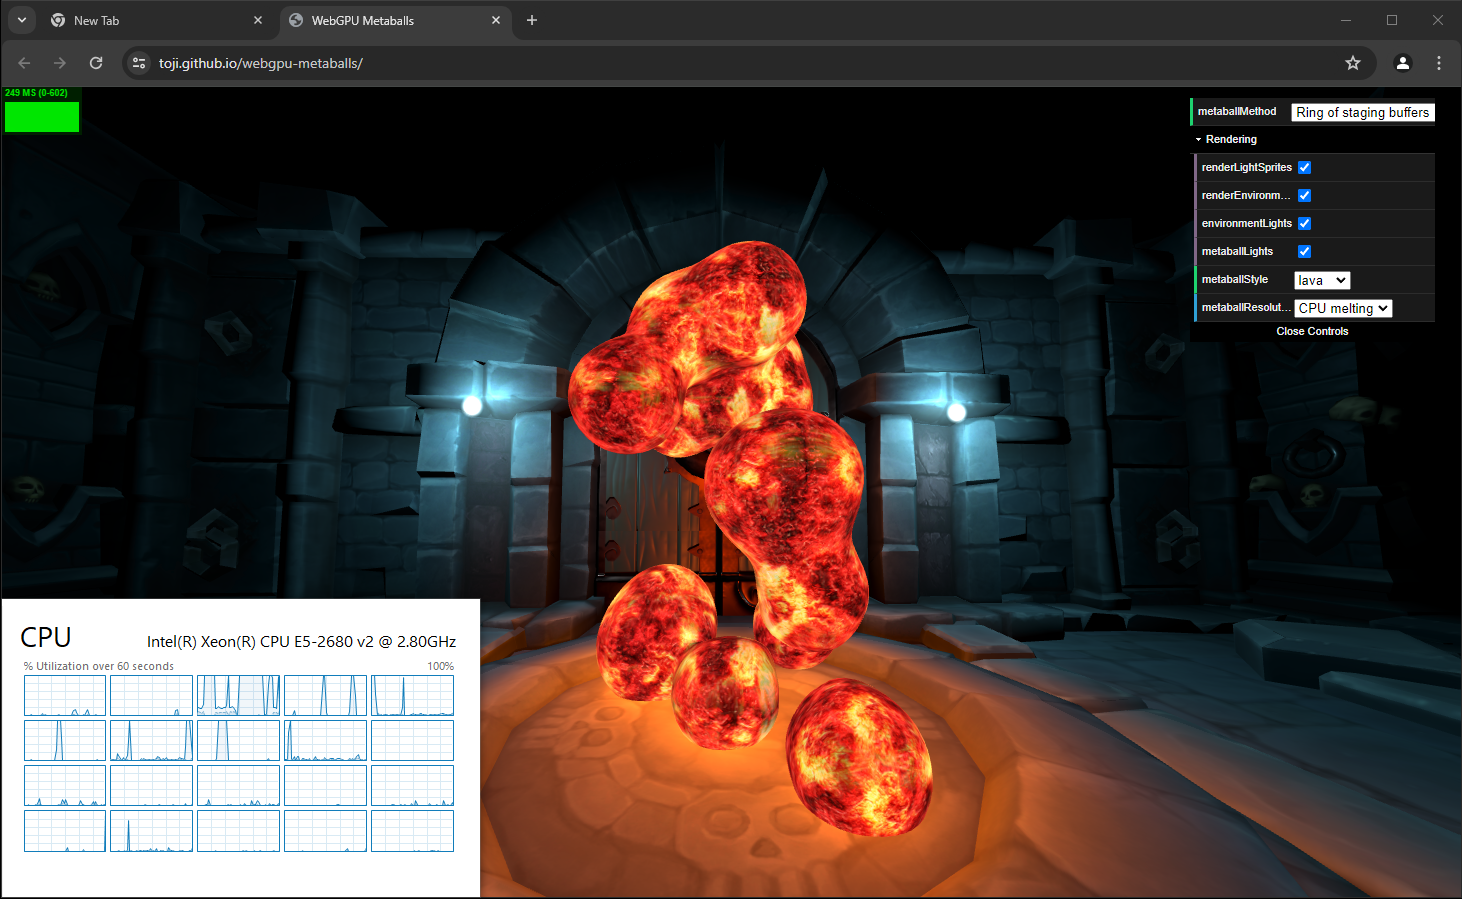
\includegraphics[width=\linewidth]{MetaBallsSimulationJS.png}
    \caption[\textit{JavaScript} implementatie van vloeistof simulatie~\autocite{Jones2024}]{
        \textit{JavaScript} implementatie van vloeistof simulatie waarbij het CPU gebruik hoog ligt en enkel kan worden uitgevoerd op een kern. \textit{JavaScript} vertraging wordt linksboven aangeduid in milliseconden~\autocite{Jones2024}.
    }
    \label{fig:MetaBallsSimulationJS}
\end{figure}

\begin{figure}
    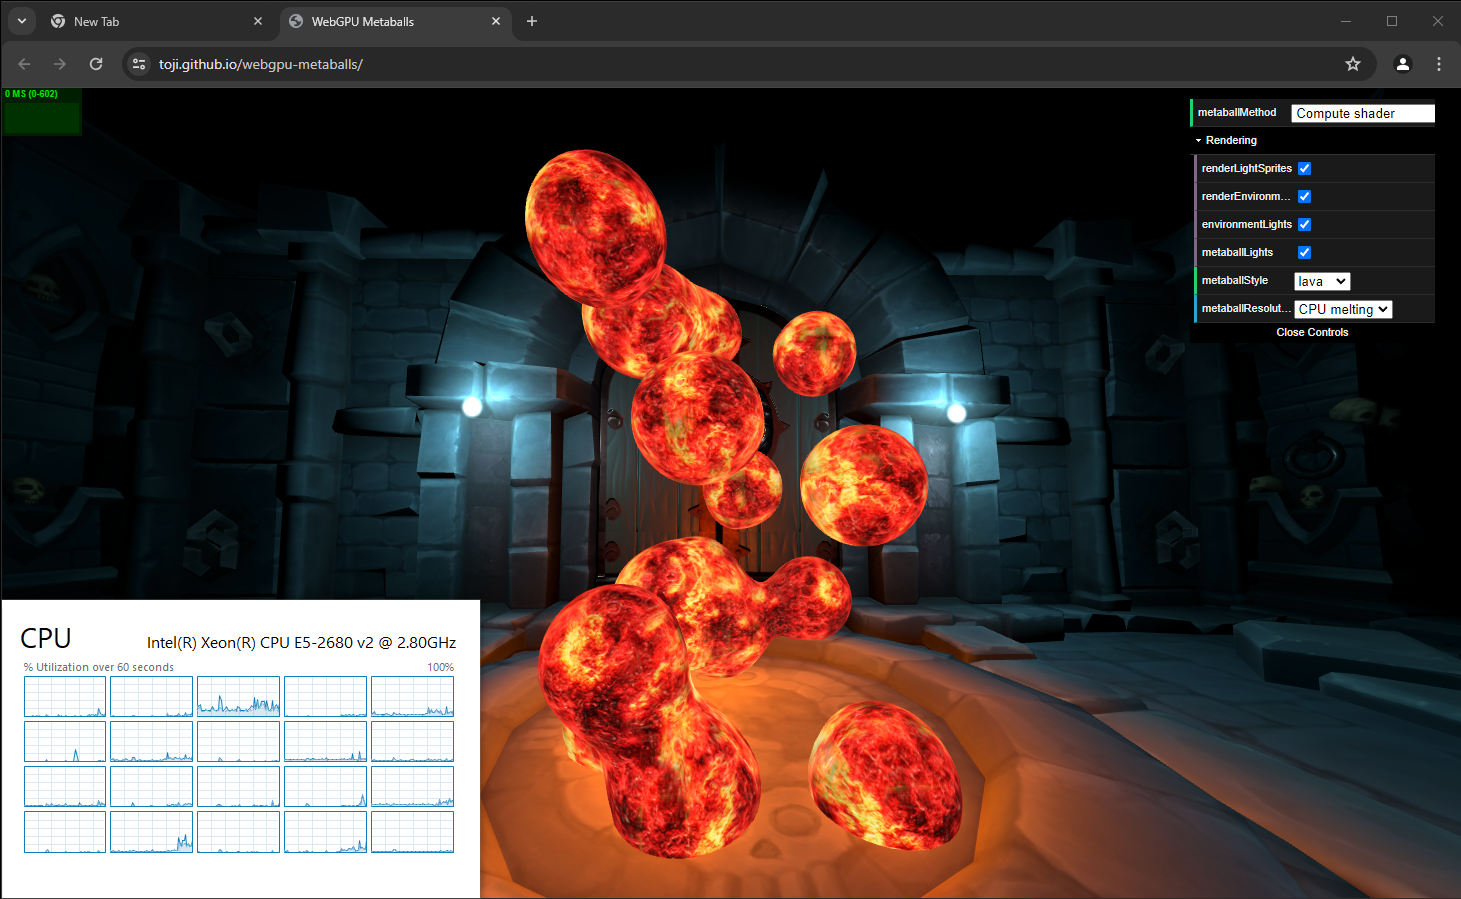
\includegraphics[width=\linewidth]{MetaBallsSimulationWebGPU.png}
    \caption[\textit{WebGPU} implementatie van vloeistof simulatie~\autocite{Jones2024}]{
        \textit{WebGPU} implementatie van vloeistof simulatie waarbij de benodigde berekeningen worden uitgevoerd op de grafische kaart. \textit{JavaScript} vertraging wordt linksboven aangeduid in milliseconden~\autocite{Jones2024}.
    }
    \label{fig:MetaBallsSimulationWebGPU}
\end{figure}

\textit{WebGPU} biedt niet enkel verbeteringen op vlak van \textit{GPGPU}. Deze technologie kan ook worden ingezet voor het produceren van individuele \textit{frames} wanneer simulaties worden uitgevoerd. Hierbij moeten zaken uit de fysica worden gesimuleerd. Implementaties aan de hand van \textit{WebGPU} laten dit opnieuw op een efficiëntere manier toe. Wanneer berekeningen voorheen werden uitgevoerd in \textit{JavaScript}, kunnen deze nu worden overgedragen aan de grafische kaart~\autocite{Wallez2023}.

\bigbreak{}

Dit kan worden gedemonstreerd aan de hand van het voorbeeld van \textcite{Jones2023}. Op afbeelding \ref{fig:MetaBallsSimulationJS} is een \textit{JavaScript} implementatie zichtbaar van het \textit{marching cubes algorithm}. Hierbij wordt een vloeistof gesimuleerd. Het interageren tussen de oppervlaktes van de bellen moet worden weergegeven. De berekeningen die hiervoor vereist zijn worden in dit voorbeeld uitgevoerd met \textit{JavaScript}. De processor wordt hierbij dus zwaar belast en dit valt zeker te merken want de simulatie begint sterk te haperen. 

\bigbreak{}

Parallelle rekenkracht met \textit{Javascript} is beperkt. Bij deze simulatie wordt zelfs maar één kern gebruikt. Dit is zichtbaar in de taakbeheer grafiek links beneden op afbeelding \ref{fig:MetaBallsSimulationJS} waarbij de processor belasting per kern wordt weergegeven. De simulatie loopt hierbij een sterke vertraging op van 250 milliseconden per \textit{frame}.

\bigbreak{}

Wanneer de instelling in dit voorbeeld echter wordt aangepast naar \textit{compute shaders} verdwijnt de \textit{JavaScript} vertraging zo goed als volledig. Dit kan worden uitgelezen op afbeelding \ref{fig:MetaBallsSimulationWebGPU}, waarbij het processor verbruik sterk is gedaald. Ook de JavaScript vertraging is gezakt naar nul milliseconden. Hierdoor kan de simulatie stabiel op 60 \textit{frames} per seconden worden uitgevoerd. En de processor wordt niet meer zwaar belast waardoor andere zaken op de webpagina \textit{responsive} blijven.

\bigbreak{}
Grafische weergave op het web werd sinds 2011 afgehandeld door \textit{WebGL}. Deze technologie was echter verouderd en werd vervangen met \textit{WebGL 2.0} in 2017~\autocite{Surma2022}. Sinds \textit{WebGL 2.0} zijn er nieuwere grafische technologieën op de markt zoals \textit{ray tracing}, waarbij individuele fotonen worden getraceerd om extreem realistische belichting te simuleren. Deze nieuwe technologieën werden niet verwerkt in \textit{WebGL} maar worden wel verwacht in \textit{WebGPU}~\autocite{Surma2022}. \textit{WebGPU} laat dus uiteraard niet enkel verbeteringen toe op vlak van \textit{GPGPU} en simulaties van realistische scenario's, maar ook voor normaal gebruik van de grafische kaart binnen de browseromgeving.

\bigbreak{}

Het is belangrijk te vermelden dat \textit{WebGPU} niet enkel vernieuwingen zal brengen in de toename van beschikbare algemene rekenkracht, maar ook de grafische prestaties verschillen tussen \textit{WebGL 2.0} en \textit{WebGPU}~\autocite{Wallez2023}. 